\documentclass{standalone}
\usepackage{pgfplots}
\pgfplotsset{compat=1.17}

\begin{document}
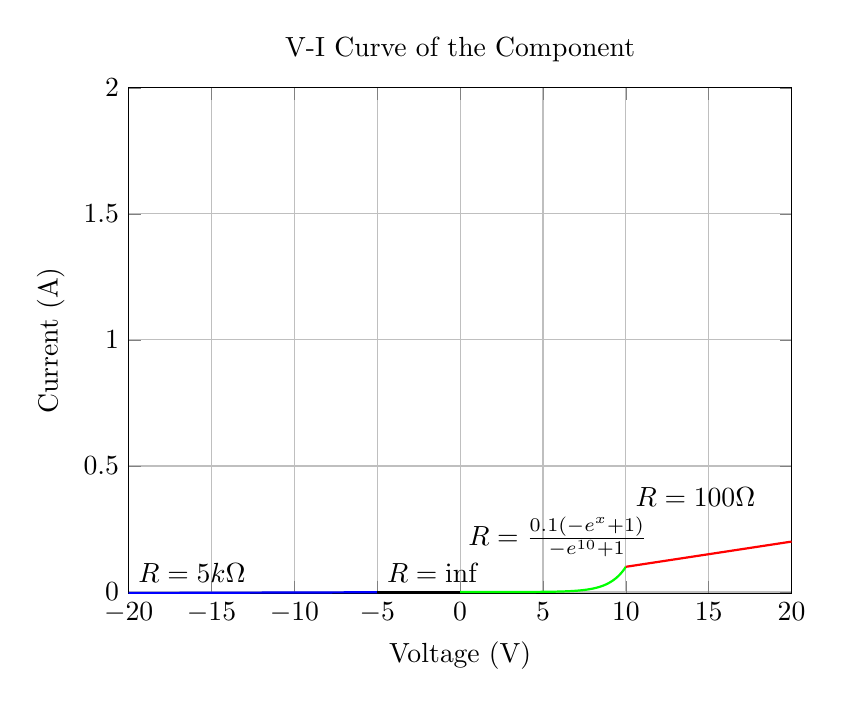
\begin{tikzpicture}
    \begin{axis}[
        width=10cm, height=8cm,
        grid=major,
        xlabel={Voltage (V)},
        ylabel={Current (A)},
        xmin=-20, xmax=20,
        ymin=-0.005, ymax=2,
        domain=-20:20,
        samples=400,
        legend pos=north west,
        title={V-I Curve of the Component}
    ]
    % Reverse region (-20V to -5V): R = 5kΩ
    \addplot[
        domain=-20:-5,
        thick,
        color=blue
    ]{x / 5000};

    % Reverse region (-5V to 0V): R = infinite
    \addplot[
        domain=-5:0,
        thick,
        color=black
    ]{0};

    % Forward region (0V to 10V): Dynamic resistance decreasing
    % NOTE: Old function used was x^2/1000 
    \addplot[
        domain=0:10,
        thick,
        color=green
    ]{(-e^(x) + 1) * ((0.1)/(-e^(10) + 1))}; 

    % Forward region (above 10V): R = 100Ω
    \addplot[
        domain=10:20,
        thick,
        color=red
    ]{x / 100};

    % Annotating key points
    \node at (-20,0) [anchor=south west] {$R = 5k\Omega$};
    \node at (-5,0) [anchor=south west] {$R = \inf$};
    \node at (-0.1,0.1) [anchor=south west] {$R = \frac{0.1(-e^{x} + 1)}{-e^{10} + 1}$};
    \node at (10,0.3) [anchor=south west] {$R = 100\Omega$};
  
    \end{axis}
\end{tikzpicture}
\end{document}
